\documentclass{article}
\usepackage{geometry}
\geometry{letterpaper}
\usepackage{doc}
\usepackage{graphicx}

\title{Peerchat: a Distributed, P2P \\ Communication Network based on Kademlia}
\author{
  Forrest Pieper\\
  Will Drevo\\
  Colin Taylor
}
\date{May 4th, 2014}

\begin{document}

\maketitle

\section{Motivation}
\label{Motivation}

Most popular online chat systems rely on a centralized authority to connect users. While these services often have very high up-time, there is no guarantee that the service providers will continue to offer their product. Additionally, these service providers can trivially gather personal data such which users chat with each other and at what frequency. \\

Peerchat is aimed to address these problems by providing a completely decentralized chat system that will remain active as long as there are individuals using the system. No individual person or organization has the ability to take the service offline. Peerchat also makes it much more difficult to track user activity since no single server (or group of servers) is likely to process every request.  

\section{Introduction}

\textit{Peerchat} is a distributed, P2P chat system based on the Kademlia DHT \cite{Maymounkov02} system which adapts Kamdelia to support persistence of users over different IP addresses, and a distributed user directory with no central server. \\

To guarantee no central dependencies, Peerchat requires that nodes bootstrap with an explicit IP address of a peer in the Peerchat network in order to be introduced into the routing table and is parameterized by the standard $k$ and $\alpha$ Kademlia parameters. \\

We implemented two main entities for each Peerchat node: \textit{User} and \textit{Node}. This separation ensures that the DHT functionality is separated from the chat protocol. 

\section{Background and Related Work}

A very similar effort is BitTorrent Chat \cite{Goldoor13}, which seeks to leverage the BitTorrent network to also also for personal, anonymous, decentralized communication. The effort has generated excitement due to the already massive user base of BitTorrent, though to date has not been released, nor is planned to be released as open-source. \\

We believe that a truly distributed chat system must be open-source in order to gain acceptance and ensure rigorous third-party audits. Though Peerchat in its current configuration is not secure, we feel that both a starting point and a commitment to open-source is important in a P2P chat client. 

\section{System}

Below is a diagram of a single Peerchat node. 

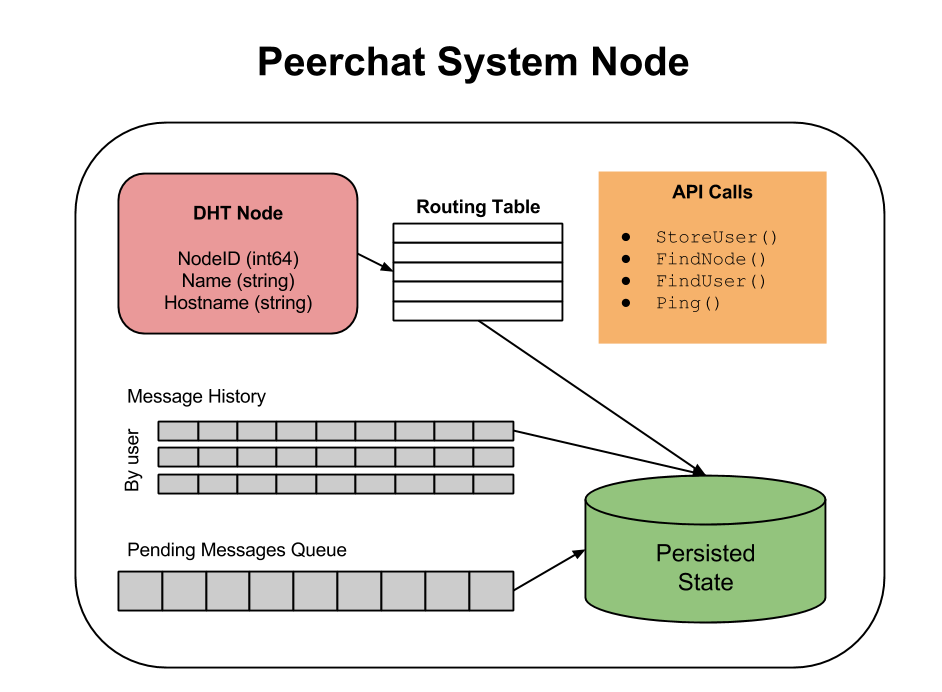
\includegraphics[scale=0.5]{peerchat}

A Peerchat user consists of a number of different routines all working together. A short description of their function is below: \\

Separate threads (goroutines):
\begin{enumerate}
	\item \textit{Message Queuing} \\
	The message queuing routine is what acts when a user submits a message. The user's node sends the message to a queue where it is stored until the Message Sender can deal with the message. Additionally, messages that are being forwarded on in the case of offline messaging are also "piggybacked" into other user's pending messages queue, and await being forwarded to other nodes. 

	\item \textit{Message Sender} \\
	The Message Sending goroutine iterates through the list of recipients with messages to be sent in the User?s queues.  Next, using the DHT, the Message Sender attempts to locate and ping the recipient peer. If the peer is online, the message is sent directly through TCP using an RPC call. If the peer is offline, the Message is sent to the K closest neighbors in the DHT by the XOR metric to increase the chances of message delivery when the recipient happens to come online. 

	\item \textit{Connection Acceptor} \\
The connection acceptor is the Peerchat routine that accepts RPC requests and spins off new goroutines to service them. 

	\item \textit{Periodic Backup} \\
	As well as backing up the system after each received message, Peerchat also backs up it?s message history, routing table, received and seen messages maps, and connection information every 30 seconds. This covers for unpopular nodes who are more often message ?forwarders? than receivers while avoiding spurious serializations to disk. 
\end{enumerate}

\subsection{Persistence}

We persist nodes' state by periodically serializing a user's routing table, messaging log, and other DHT node state to disk. When a user logs back in, we check for saved data and reconstruct the node. \\

As long as at least one of the nodes in the saved routing table is still online, the user does not have to specifiy a bootstrap node upon login.  Otherwise, the user must register their username again and provide a bootstrap node in order to rejoin the system. If the user's IP address has not changed, we relaunch the node with the old node ID. \\

If the user has a new IP address, we generate a new node ID and reorganize the routing table.
This persistence strategy minimizes system disruptions and allows nodes to seamlessly rejoin the network.

\subsection{Offline Usage}

Peerchat assumes online usage, but once a message has failed to send, falls back onto a K closest neighbors forwarding strategy. \\

Upon failure, a node also sends the message to the K nearest nodes around the node, which add the message to their background pending message queues, and attempt in their normal fashion to send them along, keeping the to/from message headers intact. This piggybacked forwarding strategy increases the chances of avoiding a situation in which both nodes continue to miss each other being online, and keeps the conversation going. 

\subsection{User Registration}

Users register when they first use Peerchat. They do this through the RegisterAndLogin function, which takes a username, ip address and ip address of a bootstrap node. In order to connect to an existing Kademlia network, the ip address of a bootstrap node is necessary. \\

Once Peerchat verifies that the bootstrap node is valid, it will create a Kademlia node, and start the Kademlia bootstrapping process (by putting the bootstrap node in it's own routing table, calling FindNode on itself to put itself in other's routing table, especially nearby nodes, and by putting its own username in the distributed hash table as well). This is done with the AnncouncePeer Kademlia API call. Once a node is registered, has created a Kademlia node, has created the infrastructure needed (data structures etc), and has bootstrapped its own and others routing tables, it it registered, logged in and in the network. \\

\subsection{User Login}

User login is a similar process to registration, except the username is known to have been in the Peerchat network at some point. As users will most likely login from the recent IP, there is a good chance that we need to do little work to get the node up and running. We must first load the user's state from persisted disk, including IP and routing table. If the IP address is the same as the last IP address login, we can keep the same node and routing table. Our routing table will be mostly the same because our XOR metric has not changed as our IP address (and hence, nodeID) has not changed. It may be stale, but the typical Kademlia protocol naturally boots out stale values. \\

If our IP address has changed, however, we must create a new Kademlia node with the hash of the IP as our new node ID. Although our distance from nodes has changed, we can still leverage the knowledge of old nodes by pinging them, and adding them to the routing table (in a different Kbucket)  if they are still online. \\

Finally, we must announce ourselves using the same bootstrapping process described above. If our IP address has changed, most of the stale username -> ip values will refresh because of Kademlia. If a stale value remains, and a sending node thinks a receiving node is in a different, old IP address, the receiving node will still receive the messages because of our offline chat protocol. Our tests reflect this. 

\section{Demonstrations}

In addition to a battery of unit tests and simulations, we also present an analysis of the Peerchat's efficiency and and performance under different parameterizations of the system. 

\subsection{Performance Testing}

We tested the Peerchat system under a exponentially increasing size of the network $n$ hosted on a single machine. \\

For this benchmark, we used our \textit{TestManyMoreRegistrations} test, which simulates a network of nodes undergoing a tumultuous increase of registrations and users entering the network. We kept $k = 10$ and $\alpha = 5$ constant, and varied only the size of the Peerchat network. 

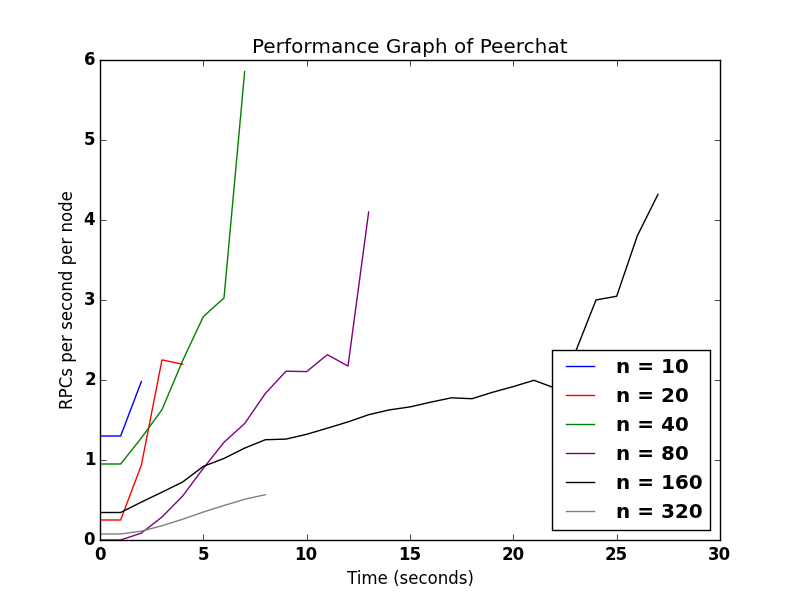
\includegraphics[scale=0.8]{performance-sweep}

We see a clear correlation between $n$ and the length of the test. Most interestingly, the rate of increase of congestion and throughput of the network \textit{decrease} as $n$ increases. \\

Unfortunately, the test of 320 nodes was cut short when our 4 core desktop could not handle the number of open files, but as you can see the slope of increase of the number of RPCs per second per node is actually the smallest of any of the tests. As the length of the tests more or less increases linearly even with the doubling values of $n$, we attribute the lower slope to the performance of the system rather than the limitations of the desktop. 

\subsection{Chat User Interface}

We considered the terminal UI secondary to the DHT implementation, as it was only a necessity for testing, but have made a usable interface for terminal users on Unix systems. \\

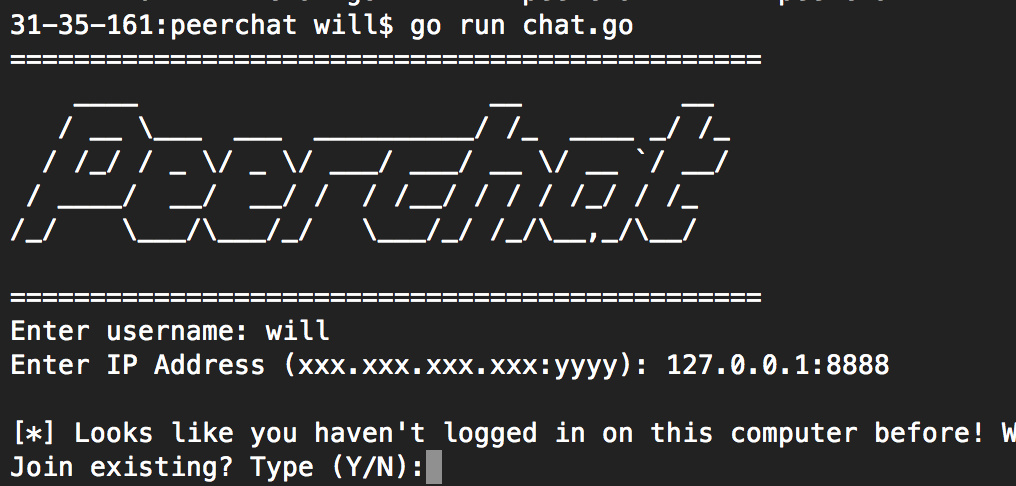
\includegraphics[scale=0.8]{ui} \\

Upon running the Peerchat script, the user is prompted to enter their username. If that username has not been logged onto the system before (if the gob backup file was not found in the Peerchat data directory), then the user is prompted to start a new network or join an existing one. 

\section{Future Work}

Peerchat has many hole that need to be filled before it becomes widely used or trusted. 

Areas of future work:
\begin{enumerate}
	\item \textit{Security} \\
	We believe that Peerchat is fundamentally ready to support a public / private key architecture. While beyond the scope of this project, the ability to encrypt messages meant for other users would make the content of messages secret, though due to the nature of forwarding, which nodes talk to each other would not be.  

	\item \textit{User Interface} \\
	Peerchat's simple user interface is definitely in need of a makeover. Even in the terminal, adapting a good $ncurses$ module from $C$ into golang would make for a more powerful and expressive interface, however a simple Qt or even web-based application would be much more convienient. 
	
\end{enumerate}

\section{Conclusion}

In conclusion, we find Peerchat to be a solid implementation of a DHT using the Kademlia protocol which is quite performant and correct under large loads. \\

Peerchat needs many improvements in order to attain wide usage, security, and absolute correctness, but we believe that ultimately open-source, P2P solutions are the way forward in a time of increasing centralization and government control. \\

It is our hope that efforts like Peerchat will inspire others to work on similar projects and provide a solid base for P2P communication development. 

\begin{thebibliography}{99}
  \bibitem{Maymounkov02}
    %Kademlia
   Maymounkov, Petar and David Mazieres
   ''Kademlia: A Peer-to-peer Information System Based on the XOR Metric''
   \textit{Peer-to-Peer Systems. Springer Berlin Heidelberg}, 2002. 53-65

  \bibitem{Goldoor13}
	%BitTorrent Chat
	Goldoor, Abe
	''Update on BitTorrent Chat.''
	\textit{The BitTorrent Engineering Blog.}, 19 Dec 2013.

\end{thebibliography}
\end {document}
